% !TEX root = ./paper.tex

\section{Physical Meaning of free energy curves and potentials of mean force}
\label{s:phys_mean}

The configurational portion of the free energy of a system is computed via the partition function

\begin{equation}
    \label{e:partition}
    Z = \int d\vec{x} \exp{-U(\vec{x}/k_B T)}
\end{equation}

as

\begin{equation}
    A = -k_B T \ln Z
\end{equation}

The integrand of Eq. \ref{e:partition} can be thought of as the unnormalized
probability, since $\mathrm{prob} \propto \exp{-U(\vec{x}/k_B T)}$.  Thus, if we wish to compute the probability distribution along an arbitrary coordinate, we would write

\begin{equation}
    \label{e:prob}
    P(x) = \frac{1}{Z} \int d\vec{x'} J(x) \exp{-U(\vec{x', x}/k_B T)}
\end{equation}

\noindent where $\vec{x'}$ is all of the degrees of freedom in the system other
than $\vec{x'}$, and $J(x)$ is the Jacobian of $x$ (see below).  The free energy curve (also called a free energy profile) along $x$ can then be computed
as

\begin{equation}
    \label{e:free}
    A(x) = - k_B T \ln(P(x))
\end{equation}


The Jacobian in Eq. \ref{e:prob} accounts for the variation in the phase space
volume associated with the differential $d\vec{x}$ with $x$.  The depends on
precisely what $\vec{x}$ is. For example, if $\vec{x} = r $ is a distance in
3-dimensional space,

\begin{equation}
J(\vec{x}) = 4 \pi r^2
\end{equation}

\noindent Physically, this means that specifying $r$ traces out a sphere of
radius $r$, and $J(r)$ is the area of that sphere.  Similarly, if $\vec{x}=
\theta$, the tilt of a vector relative to the $z$-axis, then

\begin{equation}
J(\theta) = 2 \pi \cos(\theta)
\end{equation}

which would be the arc length of the circle traced out by a unit vector for a
specific value of $\theta$.

However, it is not always convenient to work in terms of probability, since this
contains information not only about the system, but also the chosen coordinate.
To separate the two, one can also work with the probability density

\begin{equation}
    \label{e:dens}
    \rho(x) = \frac{1}{Z} \int d\vec{x'} \exp{-U(\vec{x', x}/k_B T)}
\end{equation}

\noindent
The equivalent to Eq. \ref{e:free} defines the potential of mean force (PMF)

\begin{equation}
    \label{e:pmf}
    W(x) = - k_B T \ln(\rho(x))
\end{equation}

Comparing these two quantities, it is clear that, although the terms ``PMF'' and
``free energy curve'' are often used interchangeably, they are not by definition
the same unless $J(x)=1$.  Figure \ref{f:free} demonstrates this difference for the case of a pair of ideal gase particles.

\begin{wrapfigure}{r}{6cm}
    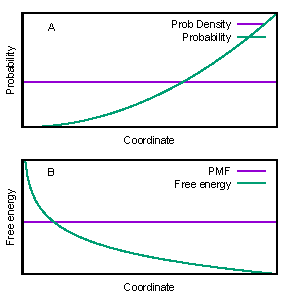
\includegraphics[width=5.8cm]{figures/ideal_gas/free}
    \caption{\label{f:free}
    Free energy curves vs. potentials of mean force.  Panel A shows the probability density and probability curves for the case where the chosen variable is the distance between 2 ideal gas particles.  The probability density is constant, while the probability increases with distance.  Panel B shows the equivalent free energy quantities, as computed by Eqs. \ref{e:free} and \ref{e:pmf}.
    }
\end{wrapfigure}

% TODO: discuss when you want PMF and when you want free energy
% TODO: discuss which methods produce what
